\section{Parallelizer Structure and Position}
\label{par_structure}
   
The auto-parallelization work done here is based on the available
OpenMP compilers, i.e. IBM\textsuperscript \textregistered XL Fortran and VisualAge\textsuperscript \textregistered C/C++. Our
auto-parallelizer is essentially a loop parallelizer.  For simplicity,
the auto-parallelizer avoids complicated parallelization constructs
and focuses on identifying and parallelizing expensive loops in the
program. The parallelizer simply marks parallelizable loops as OpenMP
\texttt{parallel do} constructs. The compiler then generates code
similar to parallel loops marked by the user. Our auto-parallelizer
does not support nested parallelization of loops unlike OpenMP.
Auto-parallelization can also be done on an OpenMP program. In this
case the auto-parallelizer skips the loop nests with OpenMP constructs
and scans for other loops that can potentially benefit from
parallelization.

\subsection{Compilation and Runtime Infrastructure}

A typical compiler and runtime structure to support OpenMP is shown in
Figure \ref{fig:runtime} \cite{Zha04}. Figure \ref{fig:linkphase}
shows the Compile and Link phases of the compiler. \emph{IR} is the
intermediate representation. The parallelizer is delayed until the
link phase of the compiler to make maximum utilization of the
inter-procedural analysis available during linking. This is shown by
the dashed lines in Figure \ref{fig:linkphase}

\begin{figure}[h]
  \begin{center}
    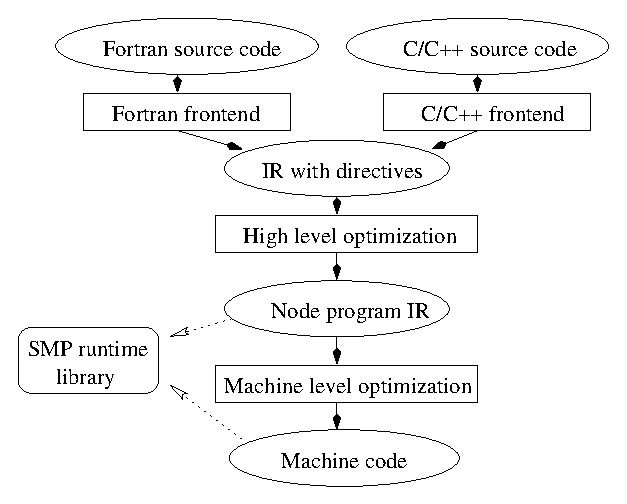
\includegraphics[angle=0, width=0.65\textwidth]{runtime.eps}
    \caption{\footnotesize Compile and runtime environment}
    \label{fig:runtime}
  \end{center}
\end{figure}


\begin{figure}[h!]
  \begin{center}
    % run boxfill.pl to get the filled version of the graph
    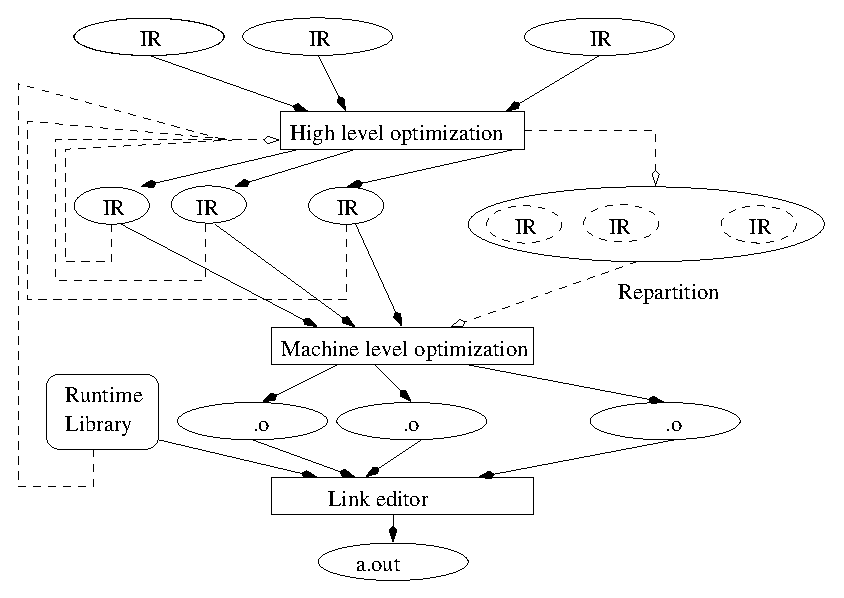
\includegraphics[angle=0, width=0.8\textwidth]{linkphase.eps}
    \caption{\footnotesize Compile and link phase optimization}
    \label{fig:linkphase}
  \end{center}
\end{figure}

SPEC2000 CPU benchmark suite was used to evaluate our techniques, as
it is one of the best indicators of the performance of the processor,
memory and compiler. Our tests focus on Spec2000FP, considering that
it is where most of the data parallel processing exists. The hardware
system used for testing in this paper is 1.1GHz POWER4\textsuperscript \texttrademark system, with 1
to 8 nodes available.

\subsection{Basic Parallelizer Structure}


{\small
\begin{algorithm}[h]
%  \SetLine %this is for setting vertical line with keyword end
  \SetKw{KwBreak}{break}
  \SetKw{KwContinue}{continue}
  \SetKwInOut{Input}{Input}
  \SetKwInOut{Output}{Output}
%  \Input{A desired loop permutation order $O=(L_1,L_2,...,L_n)$, \\
%    the original dependence matrix $\mathcal{D}$ for the loop}
%  \Output{A nearby permutation $P$}
  \BlankLine

  \Begin {
    \For {each loop nest in a procedure} {
      \For {each loop in the nest in the reverse depthfirst order (outer first)} {
        \If {the loop is user parallel} {
          \KwBreak
        }
        
        \If {the loop is marked sequential, has side-effects etc} {
          \KwContinue
        }
        
        \If {the loop has loop carried dependence} {
           try splitting the loop to eliminate dependence
           
           \If {dependence not eliminated}{
               \KwContinue
           }
        }
      
        \If {loop cost is known at compile time} {
          \If { the loop has not enough cost }
             \KwBreak
        }
        \Else {
          Insert code for run-time cost estimate
        }
        Mark this loop auto parallel \\
        \KwBreak
      }
    }
  }
  \caption{Basic loop parallelizer}
  \label{alg:parallelizer}
\end{algorithm}
}

Dependence analysis is a core part of the parallelizer. Data
\emph{dependence vectors}\cite{Ban88} are still our principal tools to
analyze and verify the transformation applied on a loop nest. Suppose
$\vec{\delta} =\{\delta_{1}\dots\delta_{n}\}$ is a hybrid
distance/direction vector with the most precise information derivable.

If we have

%It represents a \emph{data dependence} between two
%array references, corresponding left to right from the outermost loop
%to innermost loop enclosing the references. Data dependences are
%\emph{loop-independent} if the accesses to the same memory location
%occur in the same loop iteration; they are \emph{loop-carried} if the
%accesses occur on different loop iterations.


{\small
\begin{alltt}
\(L\sb{1}\)   DO i\(\sb{1}\) = 1, U\(\sb{1}\)
\(L\sb{2}\)     DO i\(\sb{2}\) = 1, U\(\sb{2}\)
         \dots
\(L\sb{n}\)       DO i\(\sb{n}\) = 1, U\(\sb{n}\)
\(S\sb{1}\)         A(\(f\sb{1}\)(i\(\sb{1}\),\(\dots\),i\(\sb{n}\)),\(\dots\),\(f\sb{m}\)(i\(\sb{1}\),\(\dots\),i\(\sb{n}\)))=\(\cdots\)
\(S\sb{2}\)         \(\cdots\)=A(\(g\sb{1}\)(i\(\sb{1}\),\(\dots\),i\(\sb{n}\)),\(\dots\),\(g\sb{m}\)(i\(\sb{1}\),\(\dots\),i\(\sb{n}\)))
\(T\sb{1}\)         B(\(u\sb{1}\)(i\(\sb{1}\),\(\dots\),i\(\sb{n}\)),\(\dots\),\(u\sb{m}\)(i\(\sb{1}\),\(\dots\),i\(\sb{n}\)))=\(\cdots\)
\(T\sb{2}\)         \(\cdots\)=B(\(v\sb{1}\)(i\(\sb{1}\),\(\dots\),i\(\sb{n}\)),\(\dots\),\(v\sb{m}\)(i\(\sb{1}\),\(\dots\),i\(\sb{n}\)))
         END DO
         \dots
       END DO
     END DO
\end{alltt}
}

as a loop nest from $L_{1}$ to $L_{n}$, we may have two dependences
$\vec{\delta}_{A}$ and $\vec{\delta}_{B}$ characterizing the nested
loops, which were caused by $S\sb{1}$/$S\sb{2}$ and
$T\sb{1}$/$T\sb{2}$, where $f$, $g$, $u$, $v$ are linear functions of
the loop induction variables. \emph{Dependence matrix}, denoted as $\mathcal{D}$, includes
$\vec{\delta}_{A}$ and $\vec{\delta}_{B}$ as two rows.

The Algorithm \ref{alg:parallelizer} shows the basic structure of the
parallelizer. The parallelizer scans through all the loop nests in a procedure
looking for parallelizable loops.  Nested parallelism is avoided by
parallelizing only one loop in every nest.  The loops in a nest are
scanned from outer to inner as outer loops have a greater benefit from
parallelization than inner loops. As a first step, loops that are not normalized and loops that are explicitly marked as sequential or have residuals, side-affects or with loop carried dependences are discarded by the parallelizer at compile time. For loops with loop carried dependences, the parallelizer tries to split the loop to eliminate the dependences. The loops are then parallelized independently. This preliminary step eliminates all non-parallelizable loops. However, naively executing all the parallelizable loops in an application may not be a good idea as we will soon discover. Parallelization is a very expensive operation with high overhead and the compiler has to be very judicial in identifying loops that can benefit from parallelization. 

This paper omits discussions about basic techniques of computing dependence matrix, privatizing scalar variables in a
loop, finding reduction variables, peeling or splitting the loop to
eliminate the loop carried dependence, etc. which are all parts of the preparation
phase for the parallelizer. We focus instead on the advanced techniques used by the parallelizer to intelligently select loops for parallelization and the optimizations that can be done after identifying a parallelizable loop. Section \ref{selection} deals with loop transformation techniques that can enhance the parallel performance of loops selected for parallelization. Section \ref{cost} explores the use of loop cost as an advanced loop selection technique for parallelization. 

